% Insert after the equal-dimensional k=8 performance comparison.
% Replace the previous k=10 feature-composition/SHAP passage if appropriate.
% Requires amsmath and graphicx; merge references.bib into your bibliography.
% Copy Picture/Fig_SHAP_TabM_K08.pdf to the manuscript's Picture folder.

At $k=8$, the two TabM RFE paths retain five common inputs:
convective available potential energy (CAPE), maximum
2-m temperature since the previous post-processing time,
K index, vertically integrated eastward water-vapour flux,
and total-column ozone.
The full-pool model additionally retains ozone mass mixing
ratio at 850~hPa, temperature at 300~hPa, and the eastward
wind component at 1~hPa.
The base-pool model instead retains surface pressure,
vertically integrated eastward ozone flux, and vertically
integrated northward heat flux.
The compact full-pool model therefore retains three
pressure-level descriptors alongside the five shared inputs.

We use SHapley Additive exPlanations (SHAP)
\cite{Lundberg2017SHAP} to examine how these inputs enter
the predictions for all 687 local test hours.
Both models remain frozen and use the same 64 randomly
sampled training hours as background references.
Attributions are approximated by averaging feature
contributions along 256 forward and reverse permutation
paths per test hour, with predictions expressed in dB
after inverse target standardization.
For each model,
\begin{equation}
\widehat{A}_h=\phi_0+\sum_{j=1}^{8}\phi_{h,j},
\label{eq:tabm_k08_shap}
\end{equation}
where $\phi_0$ is its mean prediction over the background
hours and $\phi_{h,j}$ is the attribution of input $j$.
Positive and negative attributions respectively raise
and lower the prediction relative to this reference.
Mean absolute SHAP values summarize the magnitude of
each input's influence across the test hours.

\begin{figure*}[t]
\centering
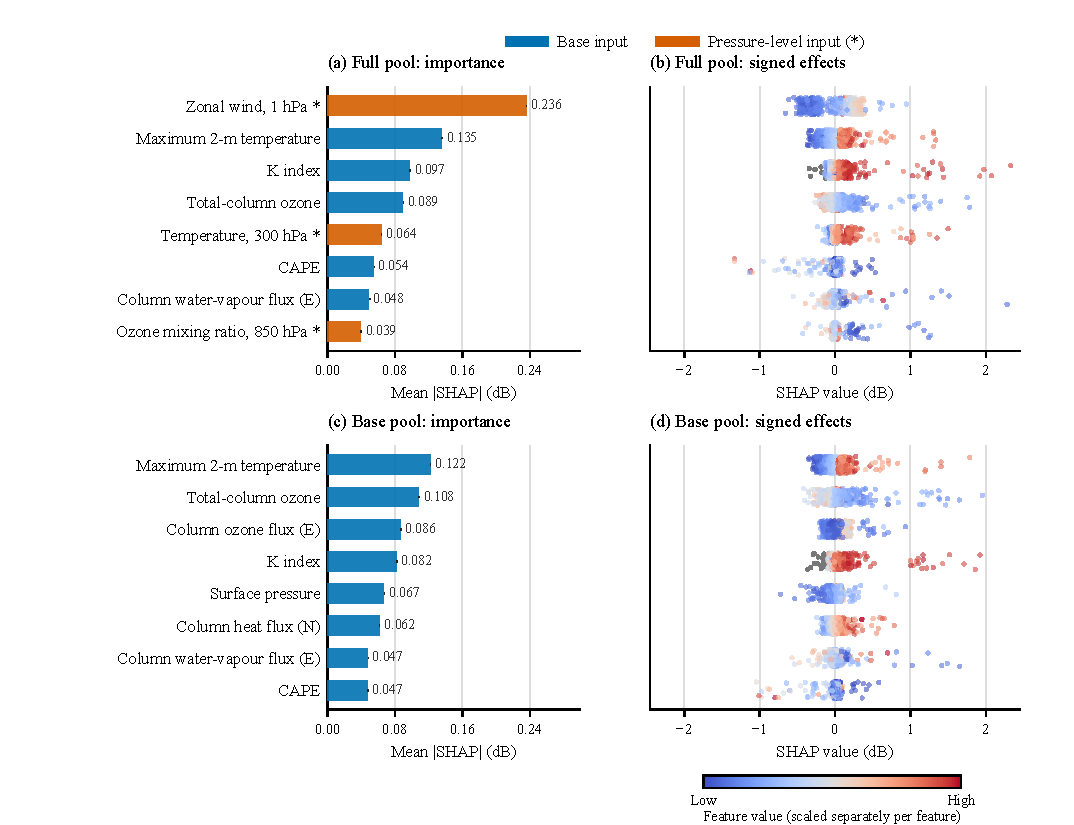
\includegraphics[width=\textwidth]{Picture/Fig_SHAP_TabM_K08.pdf}
\caption{SHAP analysis of the frozen $k=8$ TabM models
from the 156-candidate full pool and the 50-candidate
base pool, using all 687 local test hours.
(a), (c) Mean absolute attributions; thin black segments
show the range of two independent permutation replicates,
not confidence intervals.
(b), (d) Signed attributions in the corresponding row order;
each dot represents one hour.
Colour indicates the raw feature value, scaled separately
for each feature; grey dots indicate missing raw values
handled by the frozen imputer.
Orange bars and asterisks identify pressure-level inputs.
E and N denote eastward and northward components.
The two models use common axis limits, with no
attribution omitted.}
\label{fig:tabm_k08_shap}
\end{figure*}

Figure~\ref{fig:tabm_k08_shap}(a) identifies the 1-hPa
eastward wind as the most influential input of the
full-pool model, with a mean absolute SHAP value of
0.236~dB, followed by maximum 2-m temperature and
K index at 0.135 and 0.097~dB, respectively.
The other two pressure-level inputs, temperature at
300~hPa and ozone mass mixing ratio at 850~hPa,
have smaller values of 0.064 and 0.039~dB.
For the base-pool model in Fig.~\ref{fig:tabm_k08_shap}(c),
maximum 2-m temperature, total-column ozone, and
vertically integrated eastward ozone flux rank highest,
at 0.122, 0.108, and 0.086~dB, respectively.
The signed distributions in Fig.~\ref{fig:tabm_k08_shap}(b)
and (d) further show that higher maximum 2-m temperatures
and K indices generally accompany more positive
attributions in both models.
The complete importance ranking of each model is
unchanged between the two permutation replicates.
These results show that the full-pool predictor uses
both shared atmospheric descriptors and information
at specific pressure levels in its eight-input state.

The interpretation concerns the fitted prediction
functions. In particular, the leading attribution of
1-hPa wind establishes that the model relies on this
variable; it does not establish a direct attenuation
mechanism at that altitude.
Correlated atmospheric inputs can encode overlapping
weather or seasonal information, and their attributions
depend on the retained feature set and background
references. Replacing omitted inputs with background
values can also create combinations uncommon in the
observed atmosphere.
Accordingly, SHAP describes predictive associations,
while the equal-dimensional test comparison assesses
their combined predictive value. The attribution
magnitudes cannot be interpreted as physical
attenuation contributions from individual layers.
